\documentclass[tikz,border=15pt]{standalone}
\usepackage{tikz}
\usepackage{xcolor}
\usetikzlibrary{arrows.meta,calc,positioning,shapes.geometric}

\definecolor{bgcolor}{RGB}{15,23,42}
\definecolor{cardbg}{RGB}{30,41,59}
\definecolor{cardborder}{RGB}{51,65,85}
\definecolor{predborder}{RGB}{56,189,248}
\definecolor{predbadge}{RGB}{3,105,161}
\definecolor{predbg}{RGB}{23,37,84}
\definecolor{updborder}{RGB}{74,222,128}
\definecolor{updbadge}{RGB}{4,120,87}
\definecolor{updbg}{RGB}{2,44,34}
\definecolor{gainborder}{RGB}{251,191,36}
\definecolor{gainbg}{RGB}{69,26,3}
\definecolor{textblue}{RGB}{125,211,252}
\definecolor{textgreen}{RGB}{134,239,172}
\definecolor{textyellow}{RGB}{253,224,71}
\definecolor{measborder}{RGB}{244,63,94}
\definecolor{measbg}{RGB}{131,24,67}
\definecolor{inletbg}{RGB}{12,74,110}
\definecolor{outletbg}{RGB}{113,63,18}
\definecolor{outputbg}{RGB}{6,78,59}
\definecolor{purpleborder}{RGB}{192,132,252}
\definecolor{purplebg}{RGB}{59,7,100}
\definecolor{purpletext}{RGB}{233,213,255}
\definecolor{slategray}{RGB}{148,163,184}

\begin{document}
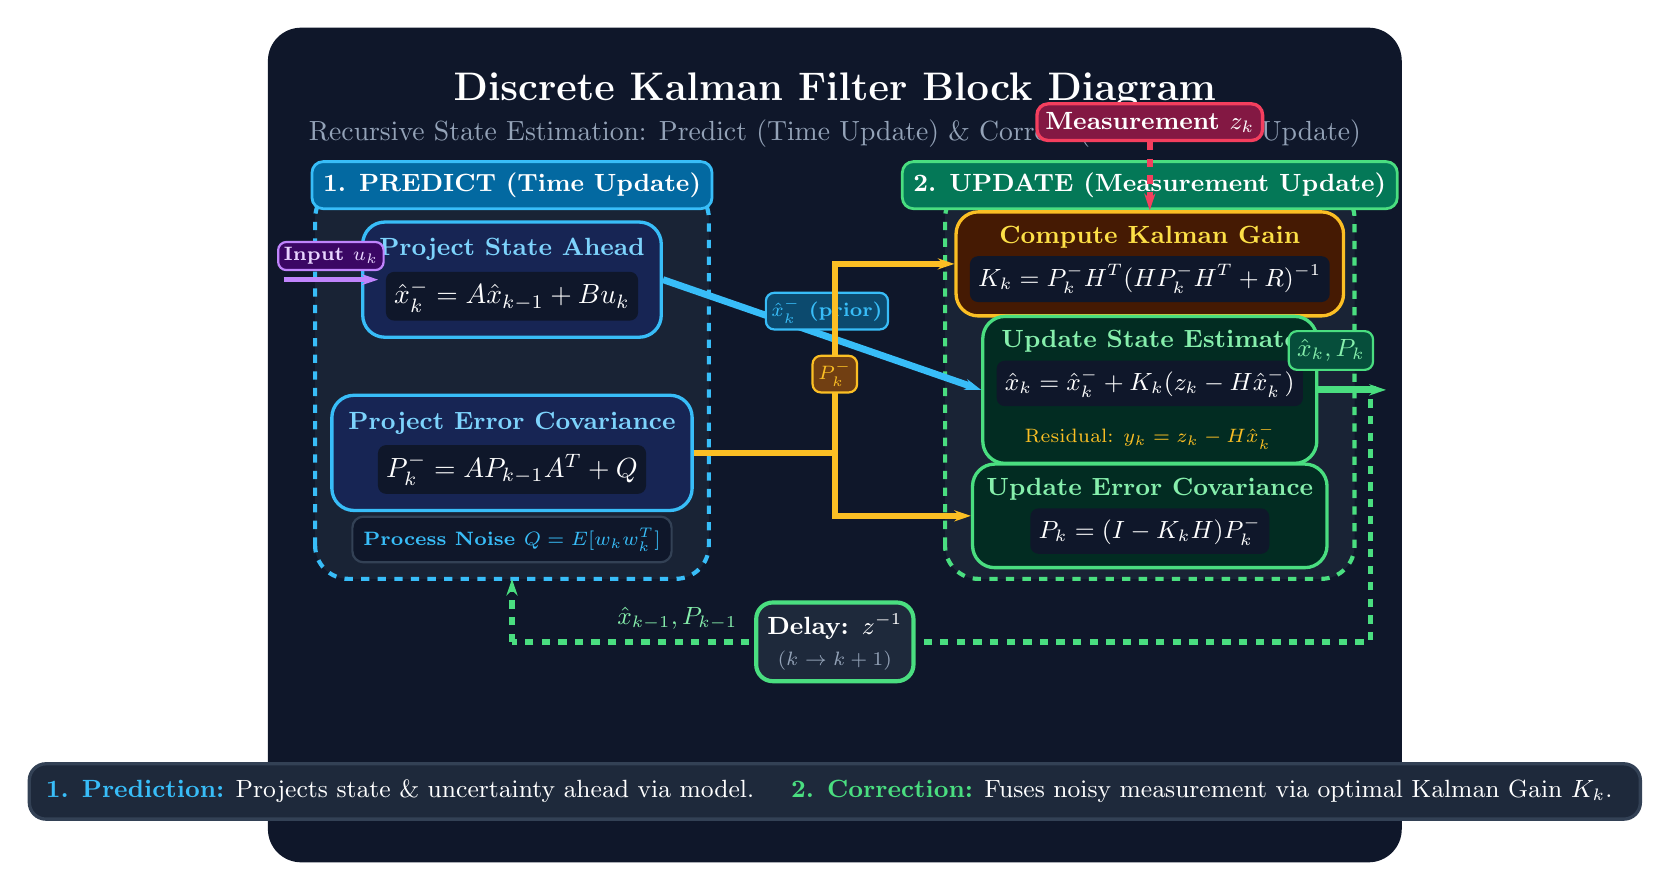
\begin{tikzpicture}[
    >={Stealth[length=6pt, width=4pt]}
]

% Background Card
\fill[rounded corners=12pt, fill=bgcolor] (-7.2,-5.4) rectangle (7.2,5.2);

% Title & Header
\node[text=white, font=\Large\bfseries] at (0, 4.4) {Discrete Kalman Filter Block Diagram};
\node[text=slategray, font=\normalsize] at (0, 3.85) {Recursive State Estimation: Predict (Time Update) \& Correct (Measurement Update)};

% 1. PREDICT REGION (Left)
\draw[predborder, dashed, line width=1.5pt, fill=cardbg, fill opacity=0.7, rounded corners=12pt] (-6.6, -1.8) rectangle (-1.6, 3.2);
\node[fill=predbadge, draw=predborder, line width=1pt, rounded corners=4pt, text=white, font=\small\bfseries, inner sep=4pt] at (-4.1, 3.2) {1. PREDICT (Time Update)};

% State Ahead Predictor
\node[fill=predbg, draw=predborder, line width=1.2pt, rounded corners=8pt, text=white, font=\small, align=center, inner sep=6pt] (STATE_PRED) at (-4.1, 2.0) {
    \textbf{\textcolor{textblue}{Project State Ahead}}\\[3pt]
    \tikz \node[fill=bgcolor, rounded corners=3pt, text=white, font=\normalsize\bfseries, inner sep=3pt] {$\hat{x}_k^- = A \hat{x}_{k-1} + B u_k$};
};

% Covariance Ahead Predictor
\node[fill=predbg, draw=predborder, line width=1.2pt, rounded corners=8pt, text=white, font=\small, align=center, inner sep=6pt] (COV_PRED) at (-4.1, -0.2) {
    \textbf{\textcolor{textblue}{Project Error Covariance}}\\[3pt]
    \tikz \node[fill=bgcolor, rounded corners=3pt, text=white, font=\normalsize\bfseries, inner sep=3pt] {$P_k^- = A P_{k-1} A^T + Q$};
};

% Process noise info
\node[fill=bgcolor, draw=cardborder, line width=0.8pt, rounded corners=4pt, text=predborder, font=\scriptsize\bfseries, inner sep=4pt] at (-4.1, -1.3) {Process Noise $Q = E[w_k w_k^T]$};

% Control input u_k
\draw[purpleborder, line width=2pt, ->] (-7.0, 2.0) -- (-5.8, 2.0);
\node[fill=purplebg, draw=purpleborder, line width=0.8pt, rounded corners=3pt, text=purpletext, font=\scriptsize\bfseries, inner sep=2pt] at (-6.4, 2.3) {Input $u_k$};

% 2. UPDATE REGION (Right)
\draw[updborder, dashed, line width=1.5pt, fill=cardbg, fill opacity=0.7, rounded corners=12pt] (1.4, -1.8) rectangle (6.6, 3.2);
\node[fill=updbadge, draw=updborder, line width=1pt, rounded corners=4pt, text=white, font=\small\bfseries, inner sep=4pt] at (4.0, 3.2) {2. UPDATE (Measurement Update)};

% Kalman Gain
\node[fill=gainbg, draw=gainborder, line width=1.2pt, rounded corners=8pt, text=white, font=\small, align=center, inner sep=5pt] (GAIN) at (4.0, 2.2) {
    \textbf{\textcolor{textyellow}{Compute Kalman Gain}}\\[2pt]
    \tikz \node[fill=bgcolor, rounded corners=3pt, text=white, font=\small\bfseries, inner sep=3pt] {$K_k = P_k^- H^T (H P_k^- H^T + R)^{-1}$};
};

% State Update
\node[fill=updbg, draw=updborder, line width=1.2pt, rounded corners=8pt, text=white, font=\small, align=center, inner sep=5pt] (STATE_UPD) at (4.0, 0.6) {
    \textbf{\textcolor{textgreen}{Update State Estimate}}\\[2pt]
    \tikz \node[fill=bgcolor, rounded corners=3pt, text=white, font=\small\bfseries, inner sep=3pt] {$\hat{x}_k = \hat{x}_k^- + K_k (z_k - H \hat{x}_k^-)$};\\[2pt]
    \textcolor{gainborder}{\scriptsize Residual: $y_k = z_k - H \hat{x}_k^-$}
};

% Covariance Update
\node[fill=updbg, draw=updborder, line width=1.2pt, rounded corners=8pt, text=white, font=\small, align=center, inner sep=5pt] (COV_UPD) at (4.0, -1.0) {
    \textbf{\textcolor{textgreen}{Update Error Covariance}}\\[2pt]
    \tikz \node[fill=bgcolor, rounded corners=3pt, text=white, font=\small\bfseries, inner sep=3pt] {$P_k = (I - K_k H) P_k^-$};
};

% Measurement Input z_k
\node[fill=measbg, draw=measborder, line width=1.2pt, rounded corners=4pt, text=white, font=\small\bfseries, inner sep=3pt] (MEAS) at (4.0, 4.0) {Measurement $z_k$};
\draw[measborder, dashed, line width=2pt, ->] (MEAS) -- (GAIN.north);

% 3. FORWARD CONNECTIONS
% Prior State Flow
\draw[predborder, line width=2.5pt, ->] (STATE_PRED.east) -- (STATE_UPD.west);
\node[fill=inletbg, draw=predborder, line width=0.8pt, rounded corners=3pt, text=predborder, font=\scriptsize\bfseries, inner sep=2pt] at (-0.1, 1.6) {$\hat{x}_k^-$ (prior)};

% Prior Covariance Flow
\draw[gainborder, line width=2pt] (COV_PRED.east) -- (0.0, -0.2);
\draw[gainborder, line width=2pt, ->] (0.0, -0.2) |- (GAIN.west);
\draw[gainborder, line width=2pt, ->] (0.0, -0.2) |- (COV_UPD.west);
\node[fill=outletbg, draw=gainborder, line width=0.8pt, rounded corners=3pt, text=gainborder, font=\scriptsize\bfseries, inner sep=2pt] at (0.0, 0.8) {$P_k^-$};

% 4. OUTPUT & FEEDBACK LOOP
\draw[updborder, line width=2.5pt, ->] (STATE_UPD.east) -- (7.0, 0.6);
\node[fill=outputbg, draw=updborder, line width=0.8pt, rounded corners=3pt, text=textgreen, font=\small\bfseries, inner sep=3pt] at (6.3, 1.1) {$\hat{x}_k, P_k$};

% Feedback line
\draw[updborder, dashed, line width=2pt] (6.5, 0.6) -- (6.8, 0.6) -- (6.8, -2.6) -- (-4.1, -2.6);
\draw[updborder, dashed, line width=2pt, ->] (-4.1, -2.6) -- (-4.1, -1.8);

% Delay Block
\node[fill=cardbg, draw=updborder, line width=1.5pt, rounded corners=6pt, text=white, font=\small\bfseries, align=center, inner sep=4pt] at (0.0, -2.6) {
    Delay: $z^{-1}$\\
    \textcolor{slategray}{\scriptsize $(k \rightarrow k+1)$}
};
\node[text=textgreen, font=\small\bfseries] at (-2.0, -2.3) {$\hat{x}_{k-1}, P_{k-1}$};

% Summary Footer
\node[fill=cardbg, draw=cardborder, line width=1.2pt, rounded corners=6pt, text=white, font=\small, align=center, inner sep=6pt] at (0, -4.5) {
    \textbf{\textcolor{predborder}{1. Prediction:}} Projects state \& uncertainty ahead via model. \quad
    \textbf{\textcolor{updborder}{2. Correction:}} Fuses noisy measurement via optimal Kalman Gain $K_k$.
};

\end{tikzpicture}
\end{document}
